
\section{Experimentation}
\label{sec:experiments}
In this section we examine the properties of \SCAMPLON{} and 
compare them to state-of-the-art random peer sampling protocols, \SCAMP{} and \CYCLON{}. 
The experiments\footnote{Implementation: https://github.com/anonymous/anonymous4now}
involve up to 100,000 nodes and are carried out on \PEERSIM{} \cite{peersim}, 
a simulator for peer-to-peer networks.
A simulation cycle is defined as $\Delta t$ in which each peer has executed its exchange protocol once.

We inspect three properties characteristic for random graphs, namely the
\emph{average shortest path length}, the \emph{average clustering coefficient},
and \emph{the partial view size distribution}. Additionally, we investigate on
\emph{robustness to random failures}.

\subsection{Clustering coefficient}

\begin{figure}
    \centering
    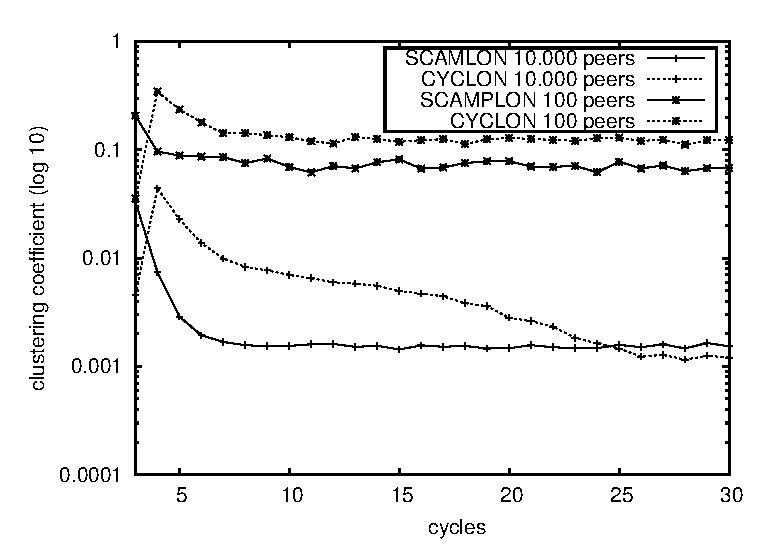
\includegraphics[width=0.49\textwidth]{img/cluster.eps}
    \caption{Clustering coefficient}
    \label{fig:clustering}
\end{figure}


\begin{asparadesc}
\item[Objective:]
    %% Highlight  
    With this experiment we want to evaluate to what degree \SCAMPLON{} generates clusters in the overlay.
    To satisfy the random peer sampling objective it is desirable that the network has very few clusters.
\item[Description:] 
   The average clustering coefficient measures the connectivity of each peer's neighborhood in the network.
  \begin{equation}
    \overline{C} = {1\over |\mathcal{N}|}\sum\limits_{x\in\mathcal{N}}C_x
    \end{equation}
    where $C_x$ is the local clustering coefficient of Peer $p_x$. The higher
    the coefficient, the more likely the network contains cliques. These
    experiments involve 100, 1000, and 10000 peers. \CYCLON{} is set to be optimal
    at 1000 peers with $|\mathcal{P}|$ set to $7$. The exchanges concern $3$
    neighbors.
\item[Results:]



\item[Reasons:]
\end{asparadesc}



\subsection{Average path length}

\begin{figure}
    \centering
    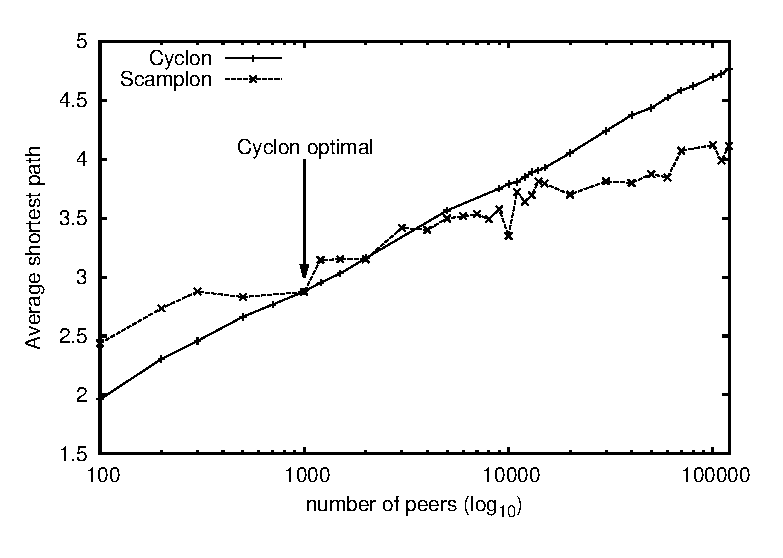
\includegraphics[width=0.49\textwidth]{img/avgpath.eps}
    \caption{Average shortest path}
    \label{fig:avgpath}
\end{figure}

\begin{asparadesc}
\item[Objective:]
\item[Description:] The average path length is the average of the shortest path
  length between peers in the graph. It counts the minimum number of hops to
  reach a peer from another given peer. The lower the value, the faster a
  message can reach the whole network.
\item[Results:]
When undersized, \CYCLON{} yield a shorter average shortest path then \SCAMPLON{}~\ref{fig:clustering}.
\item[Reasons:]
\end{asparadesc}

\subsection{Partial view size distribution}

\subsection{Resilience to failure}

\subsection{Churn}

\begin{figure}
    \centering
    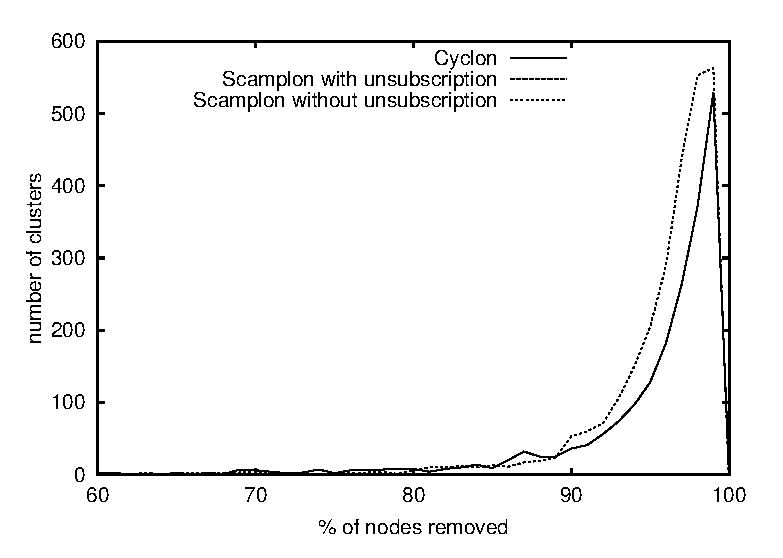
\includegraphics[width=0.49\textwidth]{img/churn.eps}
    \caption{Churn}
    \label{fig:churn}
\end{figure}

\subsection{Synthesis}

%%% Local Variables:
%%% mode: latex
%%% TeX-master: "../paper"
%%% End:
